% This file was created by tikzplotlib v0.9.1.
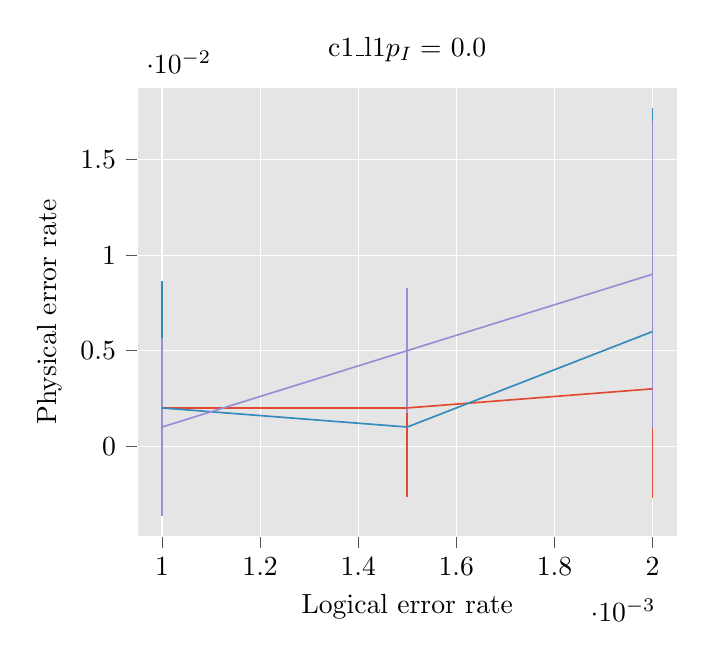
\begin{tikzpicture}

\definecolor{color0}{rgb}{0.886274509803922,0.290196078431373,0.2}
\definecolor{color1}{rgb}{0.203921568627451,0.541176470588235,0.741176470588235}
\definecolor{color2}{rgb}{0.596078431372549,0.556862745098039,0.835294117647059}

\begin{axis}[
axis background/.style={fill=white!89.8039215686275!black},
axis line style={white},
tick align=outside,
tick pos=left,
title={c1\_l1\(\displaystyle p_I = \) 0.0},
x grid style={white},
xlabel={Logical error rate},
xmajorgrids,
xmin=0.00095, xmax=0.00205,
xtick style={color=white!33.3333333333333!black},
y grid style={white},
ylabel={Physical error rate},
ymajorgrids,
ymin=-0.00471583448023164, ymax=0.0187577868077876,
ytick style={color=white!33.3333333333333!black}
]
\path [draw=color0, semithick]
(axis cs:0.001,-0.00264885169441259)
--(axis cs:0.001,0.00664885169441259);

\path [draw=color0, semithick]
(axis cs:0.0015,-0.00264885169441259)
--(axis cs:0.0015,0.00664885169441259);

\path [draw=color0, semithick]
(axis cs:0.002,-0.00269080402196845)
--(axis cs:0.002,0.00869080402196845);

\path [draw=color1, semithick]
(axis cs:0.001,0.00464885169441259)
--(axis cs:0.001,0.00864885169441264);

\path [draw=color1, semithick]
(axis cs:0.0015,0.00464885169441259)
--(axis cs:0.0015,0.00664885169441264);

\path [draw=color1, semithick]
(axis cs:0.002,0.00569080402196845)
--(axis cs:0.002,0.0176908040219685);

\path [draw=color2, semithick]
(axis cs:0.001,-0.00364885169441259)
--(axis cs:0.001,0.00564885169441259);

\path [draw=color2, semithick]
(axis cs:0.0015,0.00171111894339548)
--(axis cs:0.0015,0.00828888105660452);

\path [draw=color2, semithick]
(axis cs:0.002,0.000964105237011093)
--(axis cs:0.002,0.0170358947629889);

\addplot [semithick, color0]
table {%
0.001 0.002
0.0015 0.002
0.002 0.003
};
\addplot [semithick, color1]
table {%
0.001 0.002
0.0015 0.001
0.002 0.006
};
\addplot [semithick, color2]
table {%
0.001 0.001
0.0015 0.005
0.002 0.009
};
\end{axis}

\end{tikzpicture}
